% !TeX spellcheck = fr_FR
\chapter{Prise et manipulation}\label{ch:prise}

\paragraph*{}
Dans la culture chinoise, l'escrime et la calligraphie sont des formes d'art intimement liées et on entend communément dire qu'il faut tenir une épée comme s'il s'agissait d'un pinceau de calligraphie.
Cette affirmation semblera claire à quiconque s'est essayé à la calligraphie chinoise : pour parvenir à un bon contrôle du tracé, le pinceau doit être tenu fermement mais sans tension de manière à être relié au centre du corps du calligraphe.
La moindre faiblesse ou tension dans la prise du pinceau aura pour conséquence des traits anguleux ou hésitants.

De même, en manipulant une épée, toute tension ou faiblesse de la prise s'opposera à la fluidité des mouvements et à une connexion correcte entre l'épée et le corps, se traduisant invariablement par des mouvements d'épée maladroits et sans vie.
Pendant les assauts libres, une prise incorrecte empêche de ressentir, de s'adapter et de réagir efficacement aux mouvements de l'adversaire.

La manière de tenir la fusée déterminant la capacité à contrôler l'épée, une saisie correcte, un alignement adéquat et une attitude exempte de tensions sont les éléments fondamentaux permettant de réaliser une bonne unité avec son épée.

\section{La prise de l'épée}
De toutes les prises que j'ai pu expérimenter, je recommande particulièrement celle représentée sur la \index{prise} figure \ref{fig:prise} tant pour la pratique de la forme que pour l'assaut libre.

Pour prendre l'épée en main, alignez la gueule du tigre, le poignet et l'avant-bras dans le plan de la lame puis saisissez la partie médiane de la poignée, entre les deux viroles.
Le pouce verrouille la prise au centre de la fusée en se refermant sur l'extrémité du majeur et de l'annulaire.
L'index et l'auriculaire restent libres, participent au contrôle précis de la position de la poignée dans la main et permettent de relâcher ou resserrer la saisie.

\begin{figure}[ht]
	\centering
	\subfigure[]{\label{fig:prise}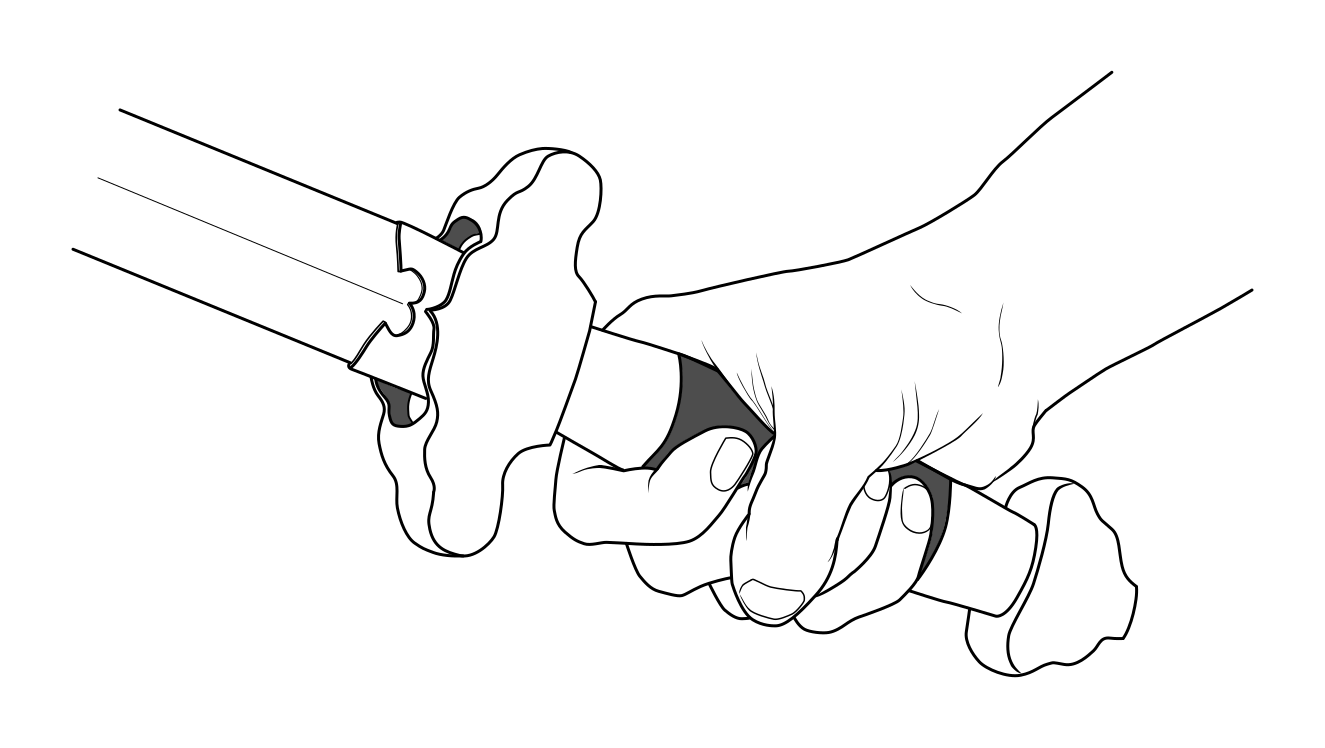
\includegraphics[width=0.69\textwidth]{../../Images/SwordGrip/sword_grip.pdf}}
	\subfigure[]{\label{fig:alignement}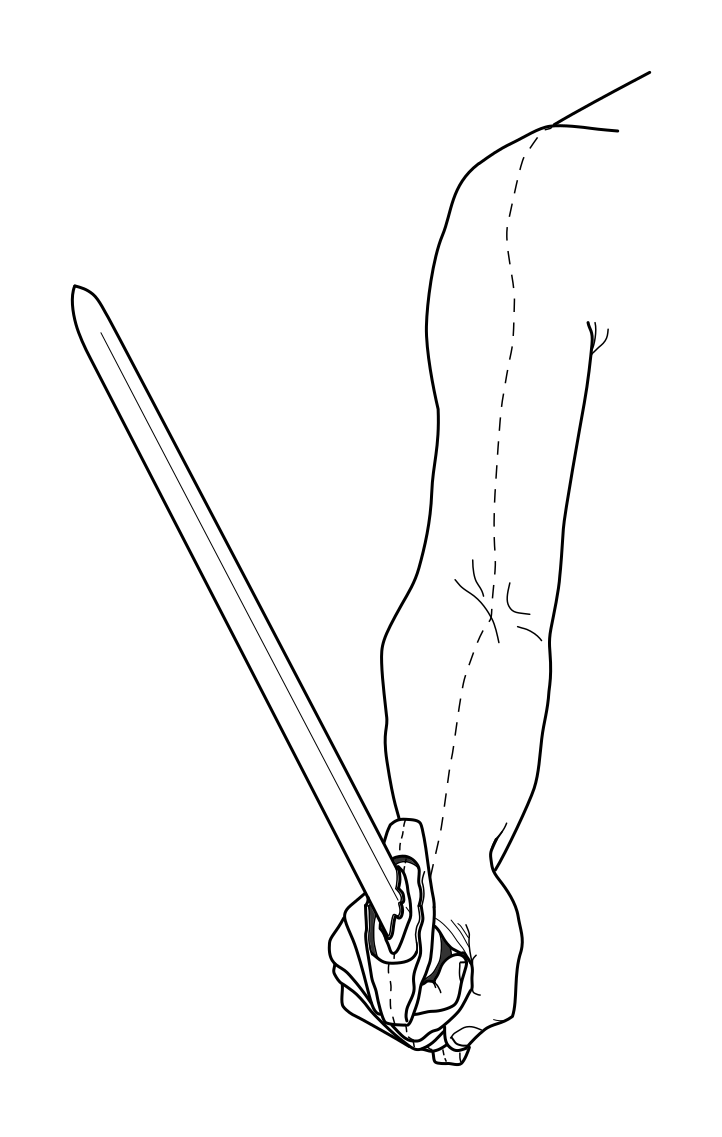
\includegraphics[width=0.29\textwidth]{../../Images/SwordGrip/alignment.pdf}}
	\caption[La prise de l'épée]{La prise de l'épée: \subref{fig:prise} la main saisit la poignée en son milieu, le pouce recouvrant le majeur et l'annulaire;
	\subref{fig:alignement} les articulations du poignet, du coude et de l'épaule sont alignées avec la lame de l'épée ainsi que représenté par la ligne en pointillés.}
\end{figure}

Comme le montre la figure \ref{fig:alignement}, le poignet, le coude et l'épaule sont situés dans le même plan que la lame.
L'épée est ainsi solidement enracinée dans la main et les centres de gravité de l'épée et du corps sont connectés, une condition essentielle pour une absorption et une expression efficaces, sans aucune tension ni contrainte sur les articulations, les muscles et tendons.
De plus, dans cette position, le coude est situé à l'intérieur de la zone de protection de la garde et ainsi, est moins exposé à des touches rapides.

\`{A} l'occasion, il est possible d'ajuster la saisie pour réaliser une technique particulière, mais il est essentiel dans ce cas de prendre garde à ne pas rigidifier ni affaiblir inconsidérément la saisie de l'épée.
En tout état de cause, lorsque les circonstances ne sont pas favorables pour un changement, ce qui est bien souvent le cas en assaut libre, il est préférable de s'en tenir à la prise principale présentée ici.

La mobilité de l'épée est également contrôlée par le resserrement ou le relâchement de la saisie. 
Il est important toutefois de garder à l'esprit que les doigts ne doivent jamais lâcher totalement la fusée : même en réalisant un moulinet, tous les doigts doivent constamment maintenir un certain contrôle de la poignée. 

Je suis convaincu qu'il est primordial de résister à la tentation de saisir la poignée au plus près de la garde, même si, la prise étant alors plus proche du centre de gravité de l'épée, celle-ci en semblerait alors moins lourde.

Tout d'abord, outre le fait que la forme en fuseau de la poignée est parfaitement adaptée à une prise centrée, dans cette prise, la garde et le pommeau sont suffisamment éloignés de la main pour ne pas gêner les mouvements de l'épée.

De plus, les gardes chinoises étant très étroites et n'enveloppant pas totalement la main comme le fait la coquille d'une rapière, elles protègent moins la main armée.
Toutefois, grâce à la position centrée de la prise, en contrôlant la lame adverse avec la garde, le pouce et l'index sont plus éloignés de la menace du tranchant adverse et donc moins exposés à des coupes fortuites que si la main est proche de la garde.

Enfin, avec une épée correctement équilibrée\index{equilibre@équilibre}, le centre de rotation résultant de cette prise centrée est précisément localisé à l'endroit permettant au pommeau de jouer pleinement son rôle dans l'équilibre dynamique de l'épée\footnote{Voyez le chapitre \ref*{ch:epeechinoise} pour de plus amples détails sur l'équilibre.}, ce qui garantit des mouvements vifs et rapides qui feront réellement la différence en assaut libre.

\section{Le sceau de l'épée}
La position de main connue sous le nom de \emph{sceau de l'épée} est assurément emblématique de la pratique de l'épée chinoise et plus particulièrement du T\`{a}ij\'{\i}j\`{\i}an.
Dans sa version traditionnelle représentée figure \ref{fig:swordfingers}, l'index et le majeur sont étendus tandis que le pouce, l'annulaire et l'auriculaire sont connectés et forment un cercle. 
Certains pratiquants utilisent aussi une version moins contrainte où le pouce, l'annulaire et l'auriculaire sont simplement relâchés sans refermer le cercle. 

\begin{figure}[ht]
	\centering
	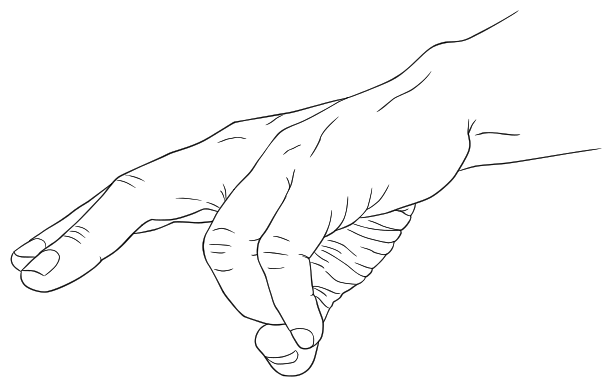
\includegraphics[width=0.69\textwidth]{../../Images/SwordFingers/SwordFingers1.pdf}
	\caption[Le sceau de l'épée]{Le sceau de l'épée}
	\label{fig:swordfingers}
\end{figure}

Le sceau a pour principal rôle de créer une spirale connectant l'extrémité du majeur gauche à la pointe de la lame et équilibrant le poids et les mouvements de l'épée.
Cette spirale est engendrée par l'extension du bras gauche dans une direction parallèle à une ligne passant par l'extrémité des deux doigts étendus.

Bien que la spirale soit aussi efficace dans les deux versions du sceau, la version traditionnelle, plus contraignante, attire beaucoup plus l'attention sur le côté gauche que ne le fait la version relâchée.

L'attention des débutants est en effet fortement focalisée sur l'épée et le côté droit, le côté gauche du corps est, le plus souvent, totalement ignoré à moins qu'ils ne soient concentrés sur le maintien strict du sceau de l'épée.
ll est donc important que les débutants n'oublient pas le sceau de l'épée en pratiquant. Ce n'est que lorsqu'ils ont acquis suffisamment d'expérience et que la spirale leur est devenue naturelle qu'ils peuvent commencer d'utiliser la forme relâchée du sceau.

\section{Manipulation}
On entend souvent répéter que l'épée doit être une extension du corps et qu'il ne faut faire qu'un avec son épée.
Ce qui peut sembler une évidence dans ce discours est toutefois loin d'aller de soi dans la pratique.
Tout d'abord, il faut considérer son épée comme un segment supplémentaire du bras, la prise de l'épée jouant le rôle d'une articulation.
Au même titre que les autres articulations, la prise doit donc être relâchée et bouger à l'unisson de tout le corps en laissant l'épée bouger librement dans la main.

En effet, si on recherche bien l'unité avec l'épée, celle-ci n'en possède pas moins sa propre individualité et une manière particulière de répondre, selon ses caractéristiques physiques, aux sollicitations du pratiquant.
Il est donc indispensable que le comportement individuel de l'épée soit pris en compte pour parvenir à harmoniser ses mouvements avec ceux du pratiquant.

Ce rapport à l'épée présente certaines similitudes avec la danse : un bon danseur en effet ne fait pas qu'imposer des pas à sa cavalière mais il est aussi capable de percevoir l'équilibre et les mouvements de celle-ci afin d'y adapter ses propres déplacements et de la conduire en douceur.
De la même manière, il ne s'agit pas d'imposer ses mouvements à l'épée mais de la guider dans la direction appropriée pour réaliser la technique souhaitée.
Les propres mouvements du pratiquant sont guidés en retour par le poids et l'élan de l'épée : si l'épée est bien une extension du corps, il n'en est pas moins vrai que le corps est lui même une extension de l'épée...
Il y a entre l'épée et le pratiquant un constant va-et-vient qui est des plus apparents dans la forme mais n'en est pas moins important en assaut libre.
De la sorte, même une épée plutôt lourde peut être manipulée efficacement et avec légèreté en utilisant le strict minimum de force musculaire, l'élan de chaque mouvement étant récupéré et réutilisé pour générer le mouvement suivant.

Le poids et l'inertie de l'épée elle même, combinés à la juste impulsion au moment opportun, apportent l'énergie nécessaire à la réalisation des techniques.
Grâce à l'inertie, le centre de gravité, emporté par l'élan de l'épée, joue le rôle d'un point d'appui permettant d'accélérer la pointe ou de la diriger vers une autre direction.
En assaut libre, les pressions exercées volontairement ou non sur la lame par l'adversaire peuvent aussi être absorbées, assimilées et transformée pour générer attaques ou ripostes.

Pour faire court, nous conclurons en disant que l'énergie est enracinée dans la fusée, qu'elle est contrôlée par le centre de l'épée et qu'elle s'exprime dans la lame.